
\documentclass[10pt,journal,compsoc]{IEEEtran}
\usepackage{listings}
\usepackage[pdftex]{graphicx}    
\usepackage{cite}
\hyphenation{op-tical net-works semi-conduc-tor}


\begin{document}

\title{Realsense Racer-bot}

\author{Jung, Myoungki}

\markboth{Localization project, Robotics Nanodegree Program, Udacity}%
{}
\IEEEtitleabstractindextext{%

\begin{abstract}
A localisation of robots is a key requirments task management for autonomous robots. Its implementation in robotics operating system provides a good starter point entering this topic.
The purpose of this report is to show the application of off the shelf localisation package inin a simulated condition, robotics operating system(ROS), its implementation, tunning parameters and results.
\end{abstract}

% Note that keywords are not normally used for peerreview papers.
\begin{IEEEkeywords}
Robot, IEEEtran, Udacity, AMCL, ROS, Localization, Racer.
\end{IEEEkeywords}}


\maketitle
\IEEEdisplaynontitleabstractindextext
\IEEEpeerreviewmaketitle
\section{Introduction}
\label{sec:introduction}

\IEEEPARstart{T}{he} localisation is a classic robotics topic with a long history and many variation. Localisation is a task with this question in mind continously.
'Where am I?' In addition, the result of localisation, space or position, is a major domain which compose of a task.
Without knowing the position of an actor, the actor cannot perform any designated task in a place. To perform a task delegated to an actor, knowing the location is a essential step and the accuracy of the evaluation also influences the success of the task greatly.
To carry out a sucessful localisation, kalman filters and a monte carlo localisation algorithm will be used from the robotics operating system packages, instead of implementing the algorithm from source code.
Wihtout positioning the robot to a desired area no other subsuent action can take place in it. Therefore, correct parameters from an adequate tuning process, a high accuracy of pose estimation will be given and this allows other tasks robot performing as intended. However, derieving a set of optimised parameter requires much knowledge on the software package, observation skill, and scientific decisions.

\section{Background}

\subsection{Kalman Filters}
Kalman filters are used in evaluation of real value from sensors with noises. Extended Kalman Filter(EKF) is prferred when the filtered data is passed to a monte carlo localisation becuase normal linear kalman filter does not allow nonlinear transformation function, and monte carlo localisation allows computation of non linear functions. 
Filteration with an extended kalman filter is a crucial action before inserting the sensor data into a localisation process pipe line as the errors in raw sensor values can propagate and amplify its magnitude greater later in localisation processes.
Therefore, filteration of noise and evaluation of near true value ensure the overall accuracy of the localisation.
\subsection{Particle Filters}
Particle filters is a common localisa     tion tool
Normal monte carlo localisation algorithm is shown in \ref{fig:mcl_algo}. 
\begin{figure}[thpb]
      \centering
      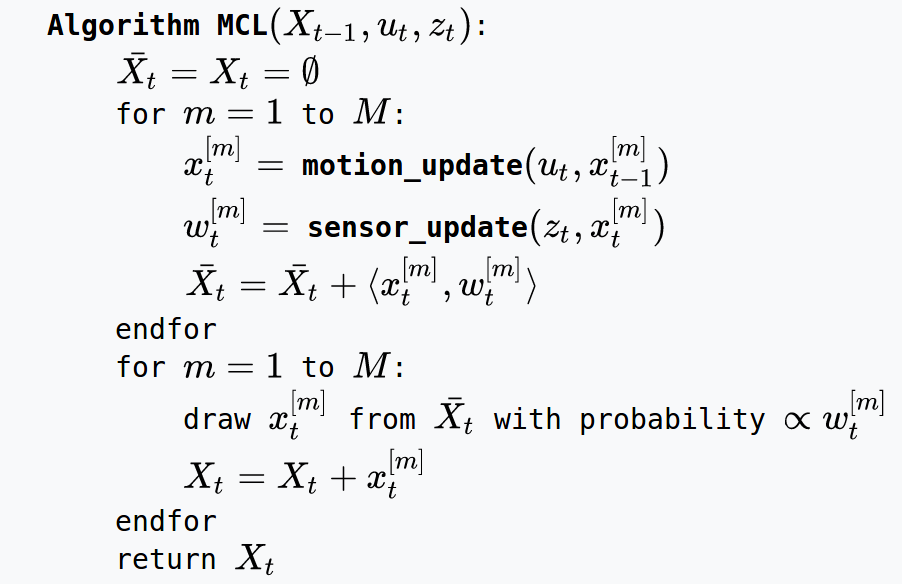
\includegraphics[width=\linewidth]{./img/mcl_algo.png}
      \caption{Algorithm of Monte Carlo localization}
      \label{fig:mcl_algo}
      \cite{Thrun2002}
\end{figure}
Adaptive (or KLD-sampling) Monte Carlo localization (AMCL)is a probabilistic localization method for a robot being position on two dimensions.\cite{Fox2001}.
KLD sampling reduced computation load by probabilistic sampling in a error range.\cite{Fox2001} This increases the performance of system performing MCL, allowing low end comuters acheive higher rate of MCL evaluation.
Allowance of algorithms to low power machines is a important trend for mobile robots recently.

\subsection{Comparison / Contrast}

The Table \ref{table:comparison_ekf_mcl} shows the comparision bewteen the extended kalman filter and monte carlo localisation in various features.
\begin{table}[ht]
      \caption{EKF vs. MCL}
      \label{table:comparison_ekf_mcl}
      \begin{center}
      \begin{tabular}{|c|c|c|}
      \hline
       & MCL & EKF \\
      \hline\hline
      Measurement types & Raw & Landmark \\
      \hline
      Measurement Noise & Any &  Gaussian \\
      \hline
      Posterior & Particles &  Gaussian \\
      \hline
      Memory Efficiency & Normal &  Good \\
      \hline
      Time Efficiency & Normal &  Good \\
      \hline
      Code difficulty & Easy &  Normal \\
      \hline
      Resolution & Normal &  Good \\
      \hline
      Robustness & Good &  No \\
      \hline
      Memory \& resolution & Yes &  No \\
      \hline
      Global localisation & Yes &  No \\
      \hline
      State space & Multimodal discrete &  Unimodal continous \\
      \hline
      \end{tabular}
      \end{center}
\end{table}


Kalman filters and particle filters can make synergy in performance and accuracy.  For a mobile robot in 2D, kalman filter can be used in embedded sensors to output less noise sensor readings to the main processing unit, and particle filters in main processing unit can utilise the noiseless sensor values to evaluate the position of the system.

\section{Simulations}
This section should discuss the performance of robots in simulation. Items to include are the robot model design, packages used, and the parameters chosen for the robot to properly localize itself. The information provided here is critical if anyone would like to replicate your results. After all, the intent of reports such as these are to convey information and build upon ideas so you want to ensure others can validate your process.
You should have at least two images here: one that shows your standard robot used in the first part of the project, and a second robot that you modified / built that is different from the first robot. Remember to watermark all of your images as well. 

\subsection{Achievements}
Both model acheived no collision and high speed driving in the circuit.

% Robot Models
\subsection{Benchmark Model}
Udacity robot with the same config and parameter was used.
\subsubsection{Model design}
\begin{figure}[thpb]
      \centering
      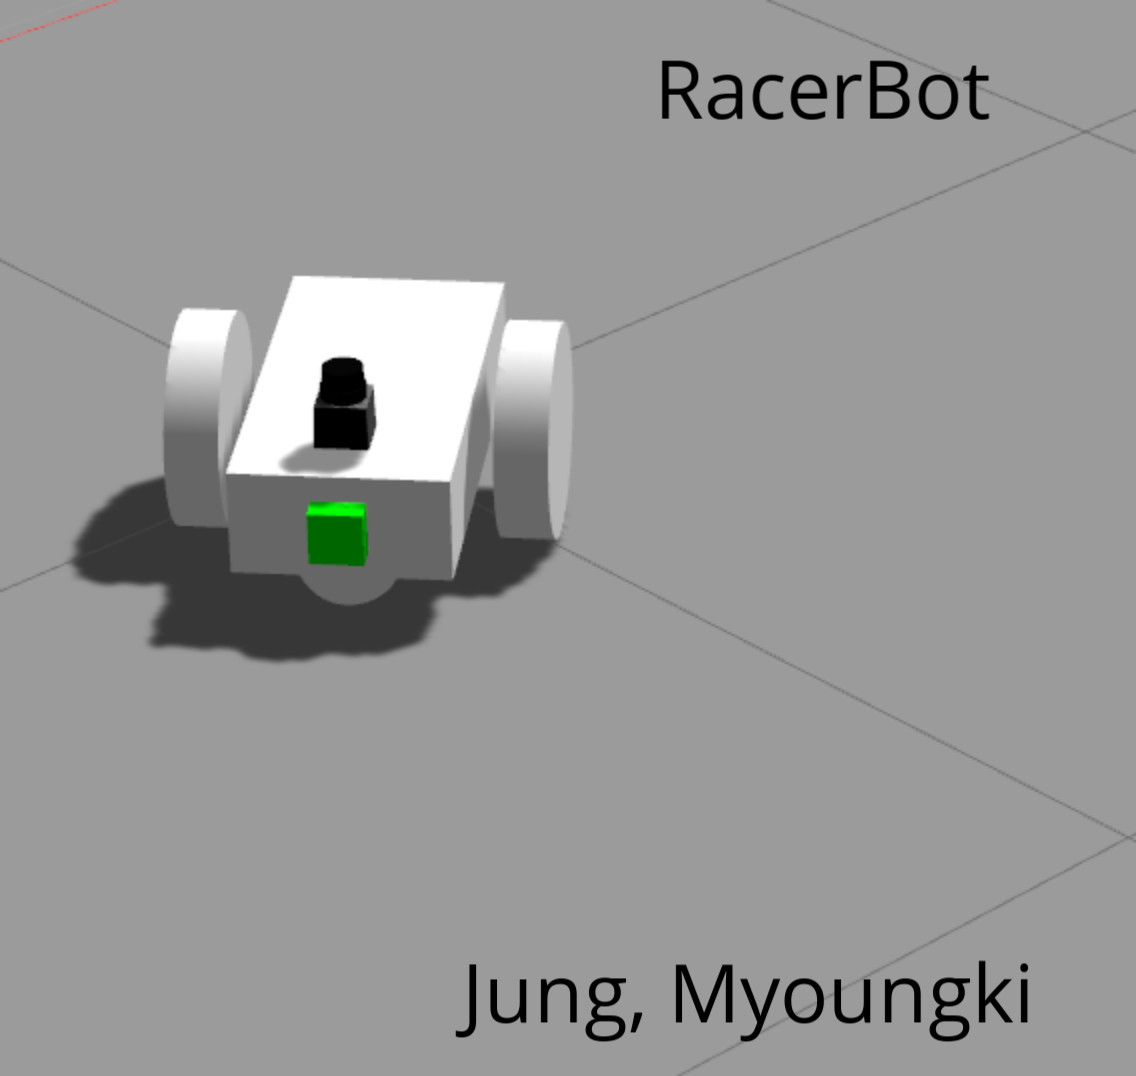
\includegraphics[width=\linewidth]{./img/udacity_bot.png}
      \caption{Personal Model Design as Guided}
      \label{fig:Basic_Model}
\end{figure}
Figure\ref{fig:Basic_Model} shows the difference to the udacitybot.

the layout and used sensors are shown in Table \ref{table:model_design}.
\begin{table}[ht]
      \caption{Model Design}
      \label{table:model_design}
      \begin{center}
      \begin{tabular}{|c|c|}
      \hline
      Atribute & Value \\
      \hline\hline
      \hline
      Size & 0.15 m by 0.10 m \\
      \hline
      Camera & RealSense D435 \\
      \hline
      LIDAR & Hokyuo  \\
      \hline
      \end{tabular}
      \end{center}
\end{table}
\subsubsection{Packages Used}
The packages used in the project should be specified as well as the topics received and published; the services it used and provided should also be addressed. 
\subsubsection{Parameters}
Localization parameters in the AMCL node should be described, as well as move\_base parameters in the configuration file. You should be able to clearly demonstrate your understanding of the impact of these parameters. The parameters from Joseph was also used for AMCL and CMakeLists.txt for navigation\_test.cpp editing techniques was found from his book.\cite{Joseph2015}
AMCL parameters were set to the values in Table\ref{table:AMCL_parameters}. To optimise the processing and the accuracy, the range of number of particles were set to 100 to 500. More than 500 only slowed down the simulation but did not result better localisation. In addition, its trigger distance was set 5 cm to 10 cm to get a reponsive localisation.
\verb!transform_tolerance! had to be low to remove warning from the console until the accuracy of localisation drops obviously.
\begin{table}[ht]
      \caption{AMCL Parameters}
      \label{table:AMCL_parameters}
      \begin{center}
      \begin{tabular}{|c|c|}
      \hline
      Parameter & Value \\
      \hline\hline \\
      \hline
      \verb!min_particles! &100 \\
      \hline
      \verb!max_particles! &500 \\
      \hline
      \verb!update_min_a! &0.1 \\
      \hline
      \verb!update_min_d! &0.05 \\
      \hline
      \verb!transform_tolerance! &0.3 \\
      \hline
      \end{tabular}
      \end{center}
\end{table}
Most of the parameters were starting from the default values, launch files, from move\_base and amcl on ROS website and experimentally increase or decrease the value slightly until a favoured result outcomes. Most of them are in the config folder of the project.\cite{AMCL_ROS} However, significant parameters in config files will be annotated on Table \ref{table:base_local_planner_parameters}.   
\begin{table}[ht]
      \caption{Cost Map Common Parameters}
      \label{table:costmap_common_parameters}
      \begin{center}
      \begin{tabular}{|c|c|}
      \hline
      Parameter & Value \\
      \hline\hline
      \verb!obstacle_range! & 1.5 \\
      \hline
      \verb!raytrace_range! & 2.0 \\
      \hline
      \verb!transform_tolerance! & 0.3 \\
      \hline
      \verb!robot_radius!& 0.15 \\
      \hline
      \verb! inflation_radius!& 0.2 \\
      
      \hline
      \end{tabular}
      \end{center}
\end{table}
Various radius and ranges were set on Table \ref{table:costmap_common_parameters}. The robot's range was limited to a range which the robot can move within 5 seconds. Calcuating larger costmap only lags the computer system and it is not so efficient.
Robot Radius was set to 0.15 and this value prevents robot bumping into wall in straight corridor and at corners. Inflation radious of costmap was determined slightly bigger than the robots turning radious. This value serves well in corners as well as near walls too. bigger value made the robot oscilating excessively. It is better to be minimal as this value.
With robot radious 0.0 or not defined, the robot tends to hit to the corner, as the path planner provides very tight corners which is surely the optimised or the shortest path. However, with out the robot radious parameter tuned robot hits to the pillar and slows down by drawing arcs around it. In addition, top speed of the robot set to 0.5, this was entirely solved and shows a easy cornering without touching the corners.


The local cost map on Table \ref{table:local_costmap_parameters} shows that the small with and height of the local cost map, low frequency of update and publish, and resolution of 0.05. The higher resulution than 0.05 did not make local map special, it only made robot wonder about more because of its resultant flat local map.
The small size of local cost map leads only 2 to 3 metres in front of the robot. This was because robot heading towards the wall during uturn as goal of a large local map points to the wall. This smaller patch only guides robot achievable local goals.
The frequency of the update and publish was lowered to optimise to the computer system. In addition, it is a set of parameter from AMCL ros website. 
\begin{table}[ht]
      \caption{Local Cost Map Parameters}
      \label{table:local_costmap_parameters}
      \begin{center}
      \begin{tabular}{|c|c|}
      \hline
      Parameter & Value \\
      \hline\hline
      \verb!update_frequency !& 5.0\\
      \hline
      \verb!publish_frequency !& 2.0\\
      \hline
      \verb!width !& 3.0\\
      \hline
      \verb!height !& 3.0\\
      \hline
      \verb!resolution !& 0.05\\
      \hline
      \verb!static_map !& false\\
      \hline
      \verb!rolling_window !& true\\
      \hline
      \end{tabular}
      \end{center}
\end{table}
The local cost map becomes indifference when the robot enters in a area without any obstacle in its sernsoring area. The contour of the cost map become flatter and the navigation stack started to make oscilation becuase the local goal is spreaded and not obvious to take. In some areas robot roams randomly or make arcs instead of following the planned path. This issue was solved by increasing the pDist twice more than gDist(default value 0.8). With pDist (3.5) and and gDist (1.5) robot tends to follow the global goal more than being lost in an uncertain local plan. This also was tweaked by the maximum speed of the robot in later section.

\begin{table}[ht]
      \caption{Global Cost Map Parameters}
      \label{table:global_costmap_parameters}
      \begin{center}
      \begin{tabular}{|c|c|}
      \hline
      Parameter & Value \\
      \hline\hline
      \verb!global_frame !& map\\
      \hline
      \verb!robot_base_frame! & \verb!robot_footprint! \\
      \hline
      \verb!update_frequency !& 5.0 \\
      \hline
      \verb!publish_frequency !& 5.0 \\
      \hline
      \verb!width !& 12.0\\
      \hline
      \verb!height !& 12.0\\
      \hline
      \verb!resolution !& 0.1\\
      \hline
      \verb!static_map !& true\\
      \hline
      \verb!rolling_window !& false\\
      \hline
      \end{tabular}
      \end{center}
\end{table}

The local cost map on Table \ref{table:global_costmap_parameters} contains the parameters used for global cost map. The global cost map did not influence as much as local map in navigation. However, a coarse boundary was set with respect to the local map. The only difference is the size and the target frame and a higer resolution. The resolution of the local cost map was set to 0.05. A higher value, more than 0.1 gave a coarse representation of action and cost anaylysis and rendered the robot roaming indecisively. However, the lower value resulted a flat, less gradient between contours of cost in the grid, and this also affected the behaivour of the robot in a similar manner with the higher value. 
In addition, it was set to staticmap.
\begin{table}[ht]
      \caption{Base Local Planner Parameters}
      \label{table:base_local_planner_parameters}
      \begin{center}
      \begin{tabular}{|c|c|}
      \hline
      Parameter & Value \\
      \hline\hline
      meter\_scoring & true \\
      \hline
      pdist\_scale & 3.5 \\
      \hline
      gdist\_scale & 2.5 \\
      \hline
      sim\_time & 1.75 \\
      \hline
      heading\_scoring & false \\
      \hline
      oscillation\_reset\_dist & 0.5 \\
      \hline
      controller\_frequency & 10 \\
      \hline
      publish\_cost\_grid\_pc & true \\
      \hline
      \end{tabular}
      \end{center}
\end{table}
Heading score was not used as it did not output good results. oscilation was set to 0.5 meter because the final parameter did not oscilate much. This was used before in the beginning of the parameter tunning because robot was circling and oscilating so much.
The parameters were iteratively detmermined, this part was the worst time wasting process in the project. Especially the computer slew significantly after some cycle and had to reboot many times to recover the responsiveness of the processes. However, using \verb!rqt_configure! could help tunning some of the \verb!move_base! and \verb!amcl! parameters.
Local Planner parameters on Table \ref{table:base_local_planner_parameters} were tunned after all cost maps are optimised because this is based on. Planner behaivour was set by \verb!pdist_scale! and \verb!gdist_scale!, persuing global goal more, the \verb!hdist_scale! was set to default 0.01.



\subsection{Personal Model}
\subsubsection{Model design}
\begin{figure}[thpb]
      \centering
      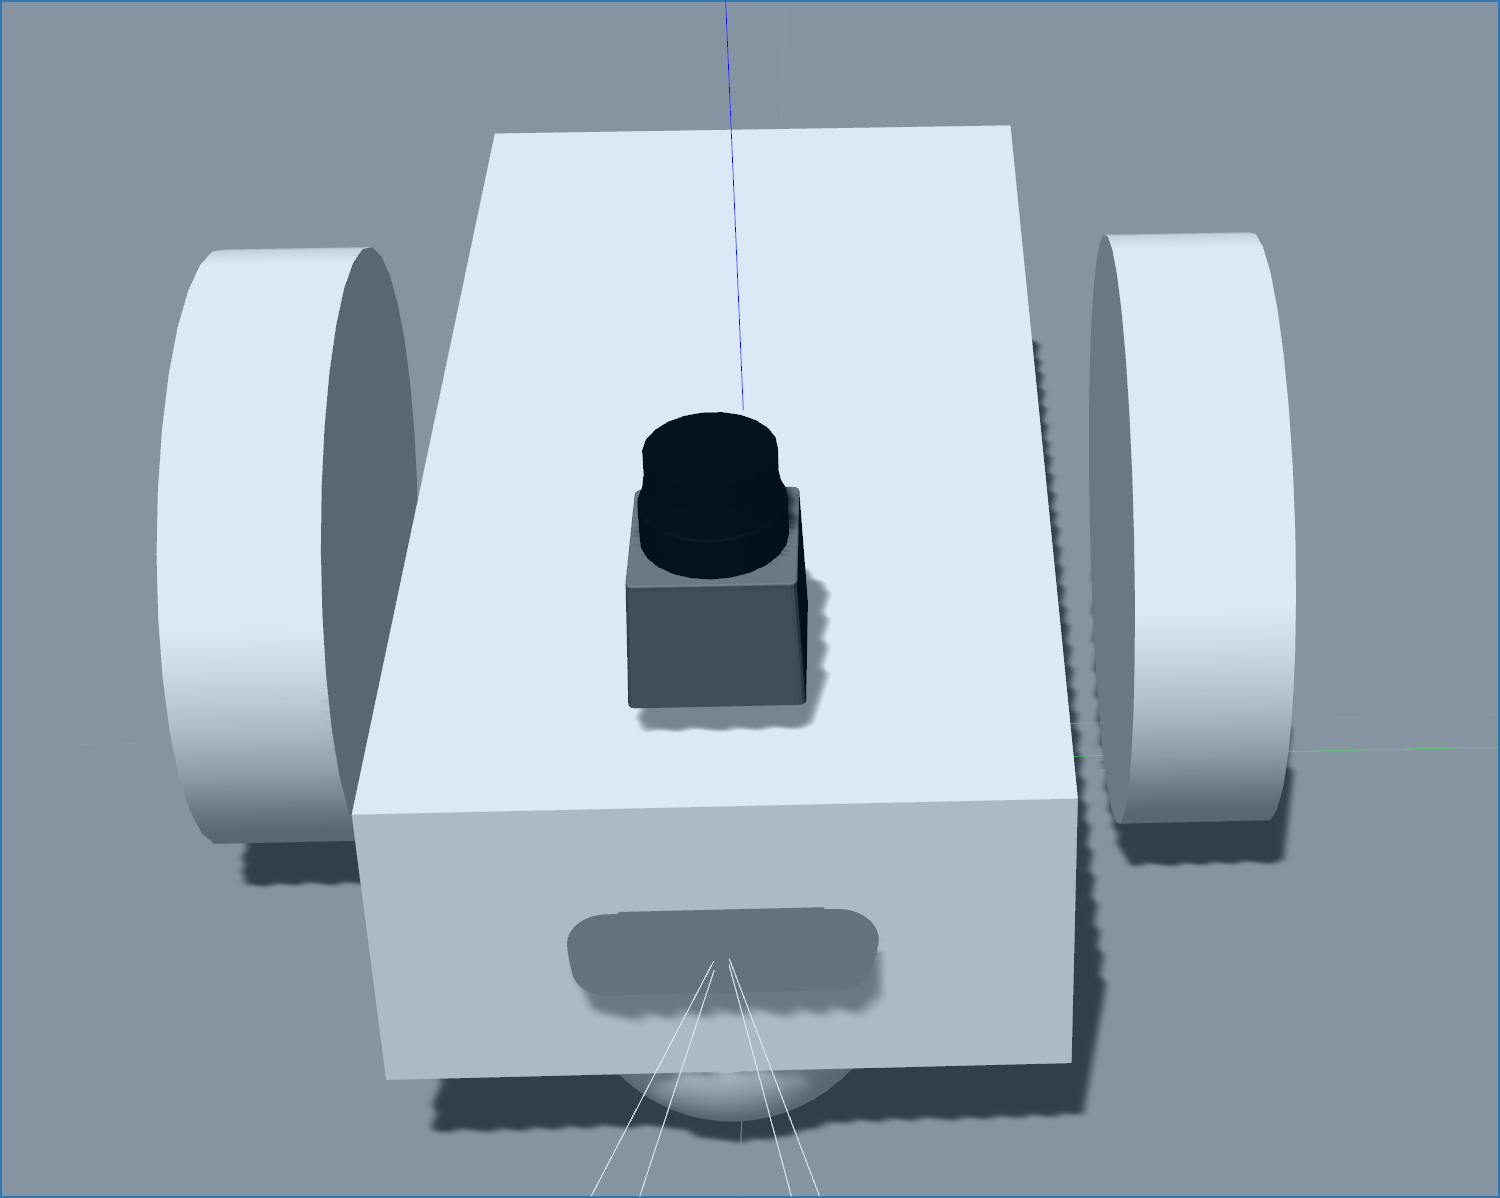
\includegraphics[width=\linewidth]{./img/racerbot.png}
      \caption{Personal Model Design with Realsense D435 mesh}
      \label{fig:Personal_Model}
\end{figure}
Figure\ref{fig:Personal_Model} shows the difference to the udacitybot.

The design of the model is the same as the udacity model. This was intended as offline vehicle for this simulation is sparkfun rebot(Figure \ref{fig:sparkfunredbot}).
The realsense camera D435 will be mounted on the front and so does the simulation model.

\begin{figure}[thpb]
      \centering
      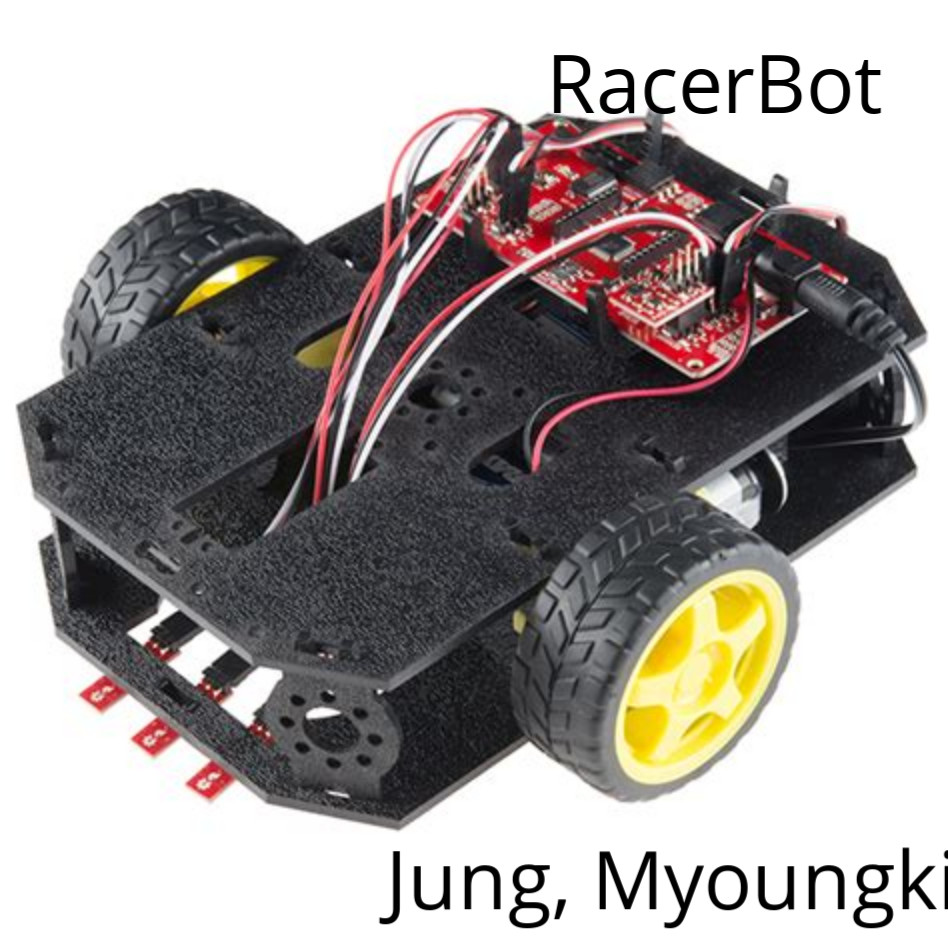
\includegraphics[width=\linewidth]{./img/sparkfunredbot.jpeg}
      \caption{Sparkfun Redbot}
      \label{fig:sparkfunredbot}
\end{figure}
\subsubsection{Packages Used}
In the simulation the same sensor was used, however, in offline model will have two proximity sensors or a generic sweeping LIDAR instead of hokyuo 1D LIDAR.
In addition, \verb!RTABMAP_ros! and \verb!realsense_gazebo_plugin! were used for the gazebo simulation and rviz.
\subsubsection{Parameters}
Basically the same as the normal udacitybot and parameters for rtabmap and realsense were added. They are defaults to the package, nothing was tuned from it. 
As the map from SLAM was not complete could not attemp to tune it. The tuning can be done more when I learn more about RTABMAP later in this course.

\section{Results}
Both robot with and without RTABMAP arrives to the goal at same time frame, 30 seconds wall time, without crashing to the wall or corner because it uses the same chassis and the same parameters.
m
\begin{lstlisting}[language={[Sharp]C}, caption={racerbot launch command},label={list:Racerbotlaunch}]
      roslaunch slam_project main.launch
\end{lstlisting}
The default racer bot simulation can be launched by the command shown in Listing \ref{list:Racerbotlaunch}.
Present an unbiased view of your robot's performance and justify your stance with facts. Do the localization results look reasonable? What is the duration for the particle filters to converge? How long does it take for the robot to reach the goal? Does it follow a smooth path to the goal? Does it have unexpected behavior in the process? \\
For demonstrating your results, it is incredibly useful to have some watermarked charts, tables, and/or graphs for the reader to review. This makes ingesting the information quicker and easier.
\subsection{Localization Results}

The Figure \ref{fig:goal_arrival} shows the robot can reach the goal by itselft. The pose array is densely populated right infront of the robot, not on the centre of inertia. However, this does not cause any trouble in navigation and collision avoidance.
\begin{figure}[thpb]
      \centering
      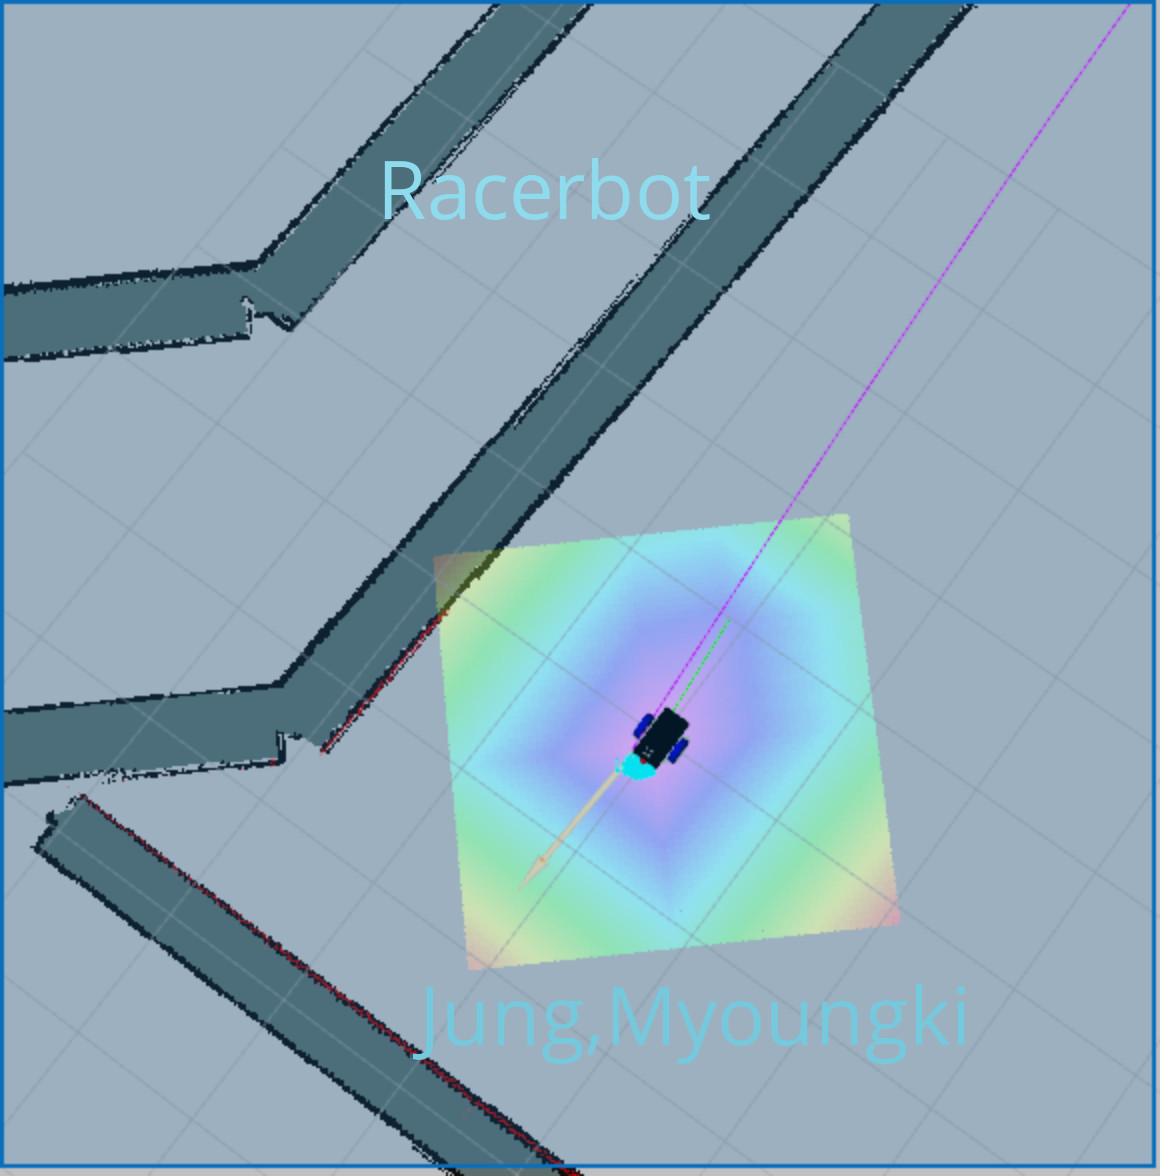
\includegraphics[width=\linewidth]{./img/goalarrival.png}
      \caption{Arrival to the goal}
      \label{fig:goal_arrival}
\end{figure}
The orange arrow represents the current goal pose, the violet line is the NavFPath of ROS, a short green line is the local path, and the rainbow box shows the coloured heat map of total cost. 
The Figure  \ref{fig:goalconsole} shows that the robot arrived to the 
\begin{figure}[thpb]
      \centering
      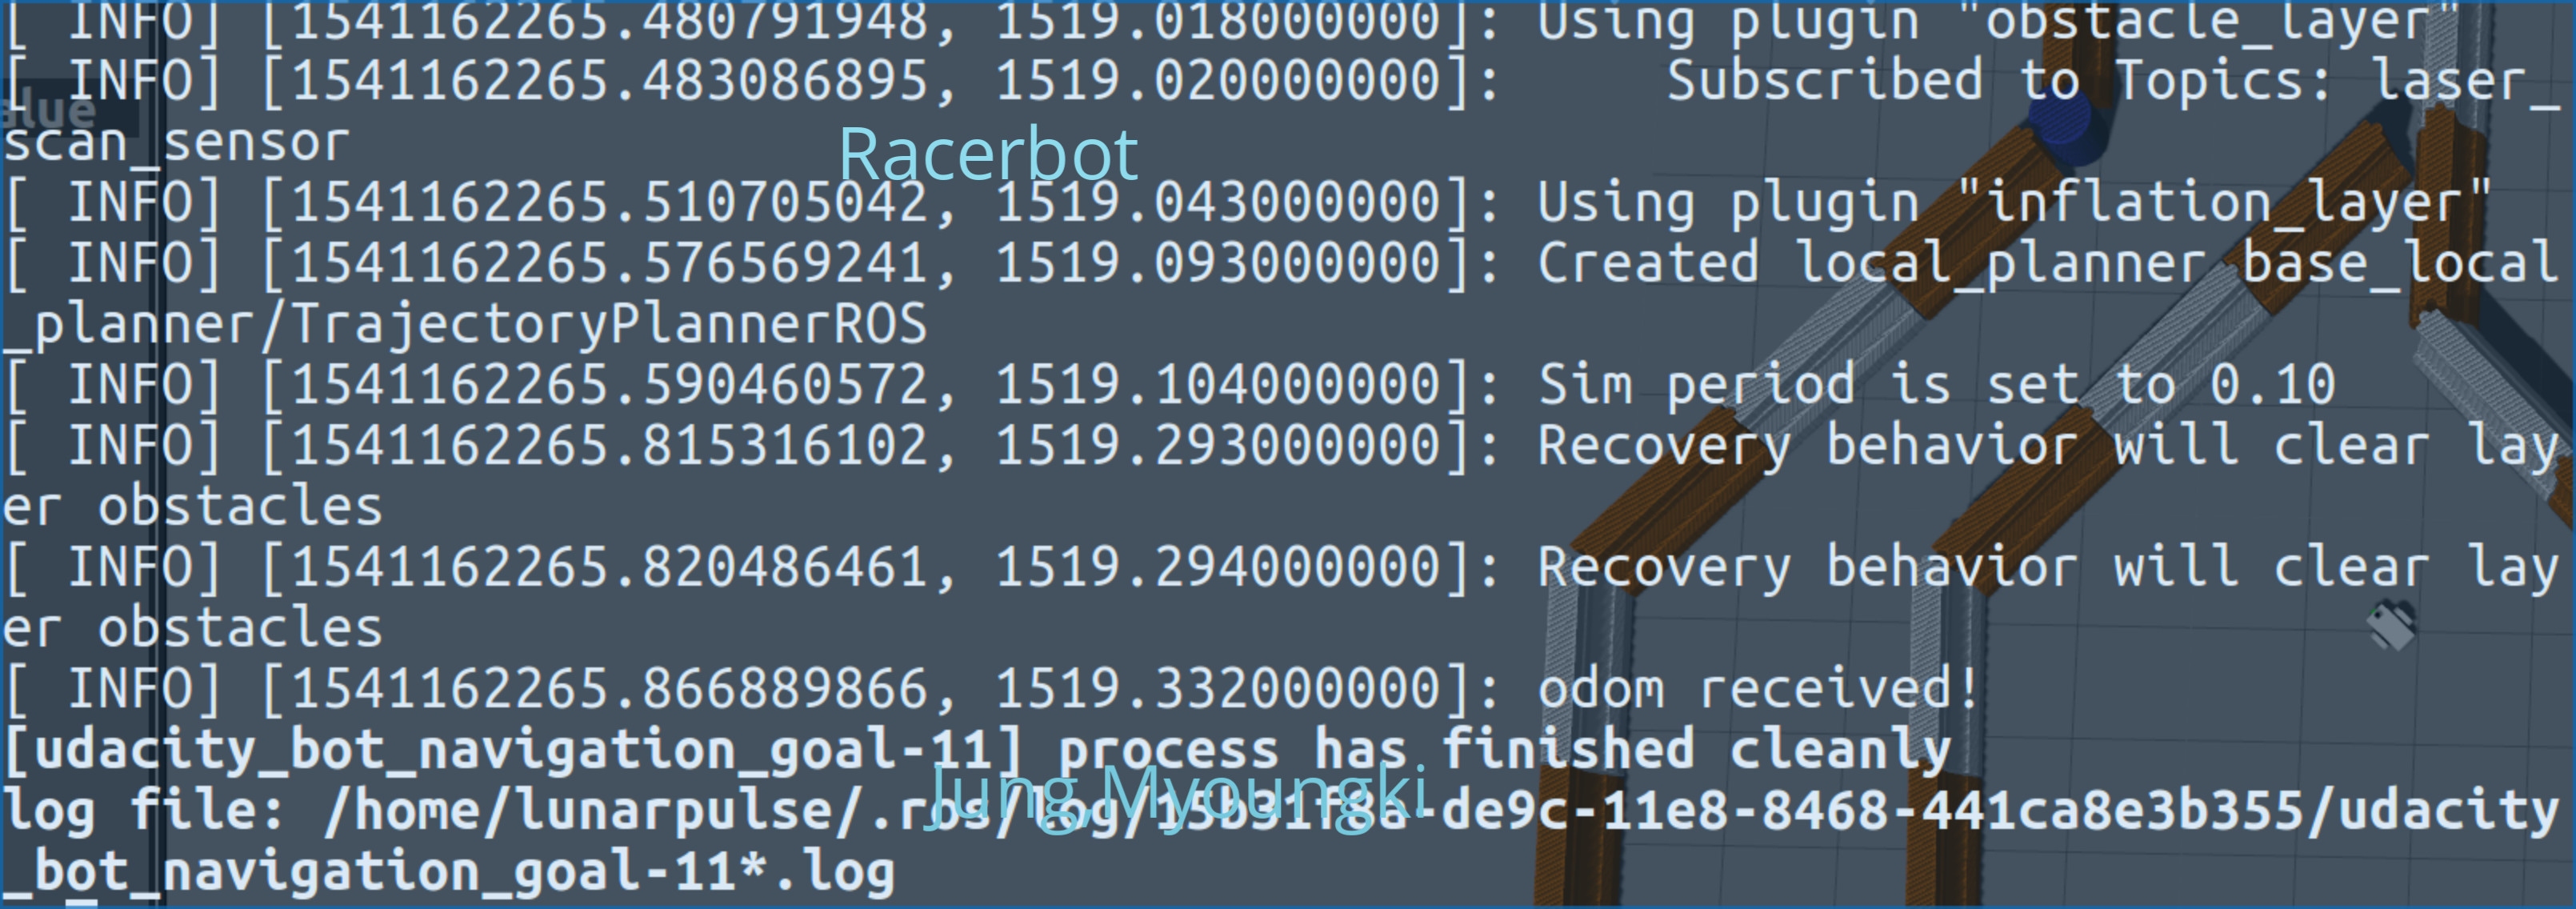
\includegraphics[width=\linewidth]{./img/goalconsole.png}
      \caption{Arrival to the goal}
      \label{fig:goalconsole}
\end{figure}
In the figure, local cost map is relatively flat because no obstacles inside the local cost map because The total cost function is dependent on the sensored obstacles and the certainty of mcl localisation and the result cost map becomes indifferent. 
Figure \ref{fig:localcostmap} shows the local cost map with an array of obstacle in the scene, the contour of cost map is more steep and shows the prefered heading of the robot as bright purple, red is the opposite direction. In addition, there is a slight descripency between local path and global navigation path. the robot is following in between two path, and sometimes runs off the route before and after a narrow curve. The Figure \ref{fig:localcostmap} shows a recovery of its heading from a U-turn.
\begin{figure}[thpb]
      \centering
      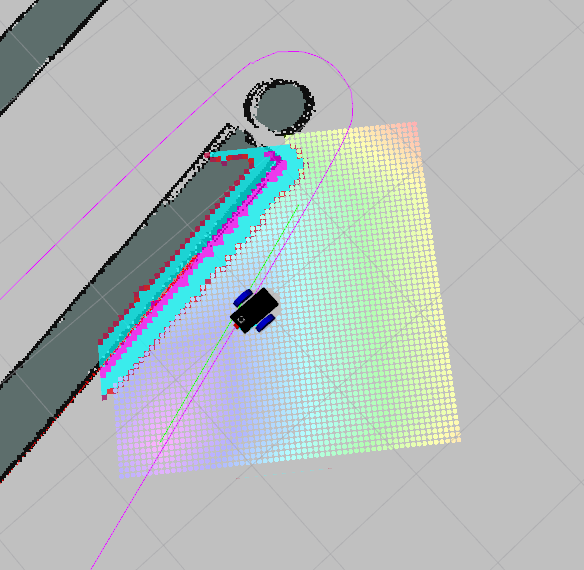
\includegraphics[width=\linewidth]{./img/localcostmap.png}
      \caption{Local cost map with obstacle existing on one side}
      \label{fig:localcostmap}
\end{figure}
In this project, my personal choice of sensor, realsense d435 was used as the author believe that a depth camera, like kinect, can provide much richer information to the robot.
The \verb!realsense_gazebo_plugin! was installed outside of the project source code and integrated.\cite{Missri}
In adition, RTABMAP ros package was used to process the data from the depth camera simulation. As the realsense d435 was supported officially by RTABMAP, integrateion of the packages were striahg forward. 
The entire packages can be run by the shell code below Listing \ref{list:RTABMAPracerbotlaunch}.

\begin{lstlisting}[language={[Sharp]C}, caption={RTABMAP integrated racerbot launch command},label={list:RTABMAPracerbotlaunch}]
roslaunch slam_project main_rtatslam.launch
rtabmap_args:="--delete_db_on_start" 
depth_topic:=/realsense/camera/depth/image_raw
rgb_topic:=/realsense/camera/color/image_raw
camera_info_topic:=/realsense/camera/color/camera_info
      odom_topic:=/odom
\end{lstlisting}

The result of this command shows in Figure \ref{fig:slam_project_DepthCloud}.
\begin{figure}[thpb]
      \centering
      \includegraphics[width=\linewidth]{./img/slam_project_DepthCloud.png}
      \caption{Realsense Depth Cloud in front of the robot}
      \label{fig:slam_project_DepthCloud}
\end{figure}
The Figure \ref{fig:rtabslam_racerbot} entire screen showing Rviz and RTABRviz. The top left is the RTABMAPRviz from RTABMAP package and it shows the result of mapping in its main screen. The bottom left terminal shows many warnings of lack of \verb!odom_info! and not enough keys. As the \verb!odom_info! is not available in the simulation, the accuracy of the mapping is not as great as it supposed to be because the package highly depends on odm info. When it was tested with Realsense D435 camera, it provided fairly accurate maps on the fly with in 1 metre from the object. D435 tends to provide fluctuating surface in a long distance, more than 3 metres.

\begin{figure}[thpb]
      \centering
      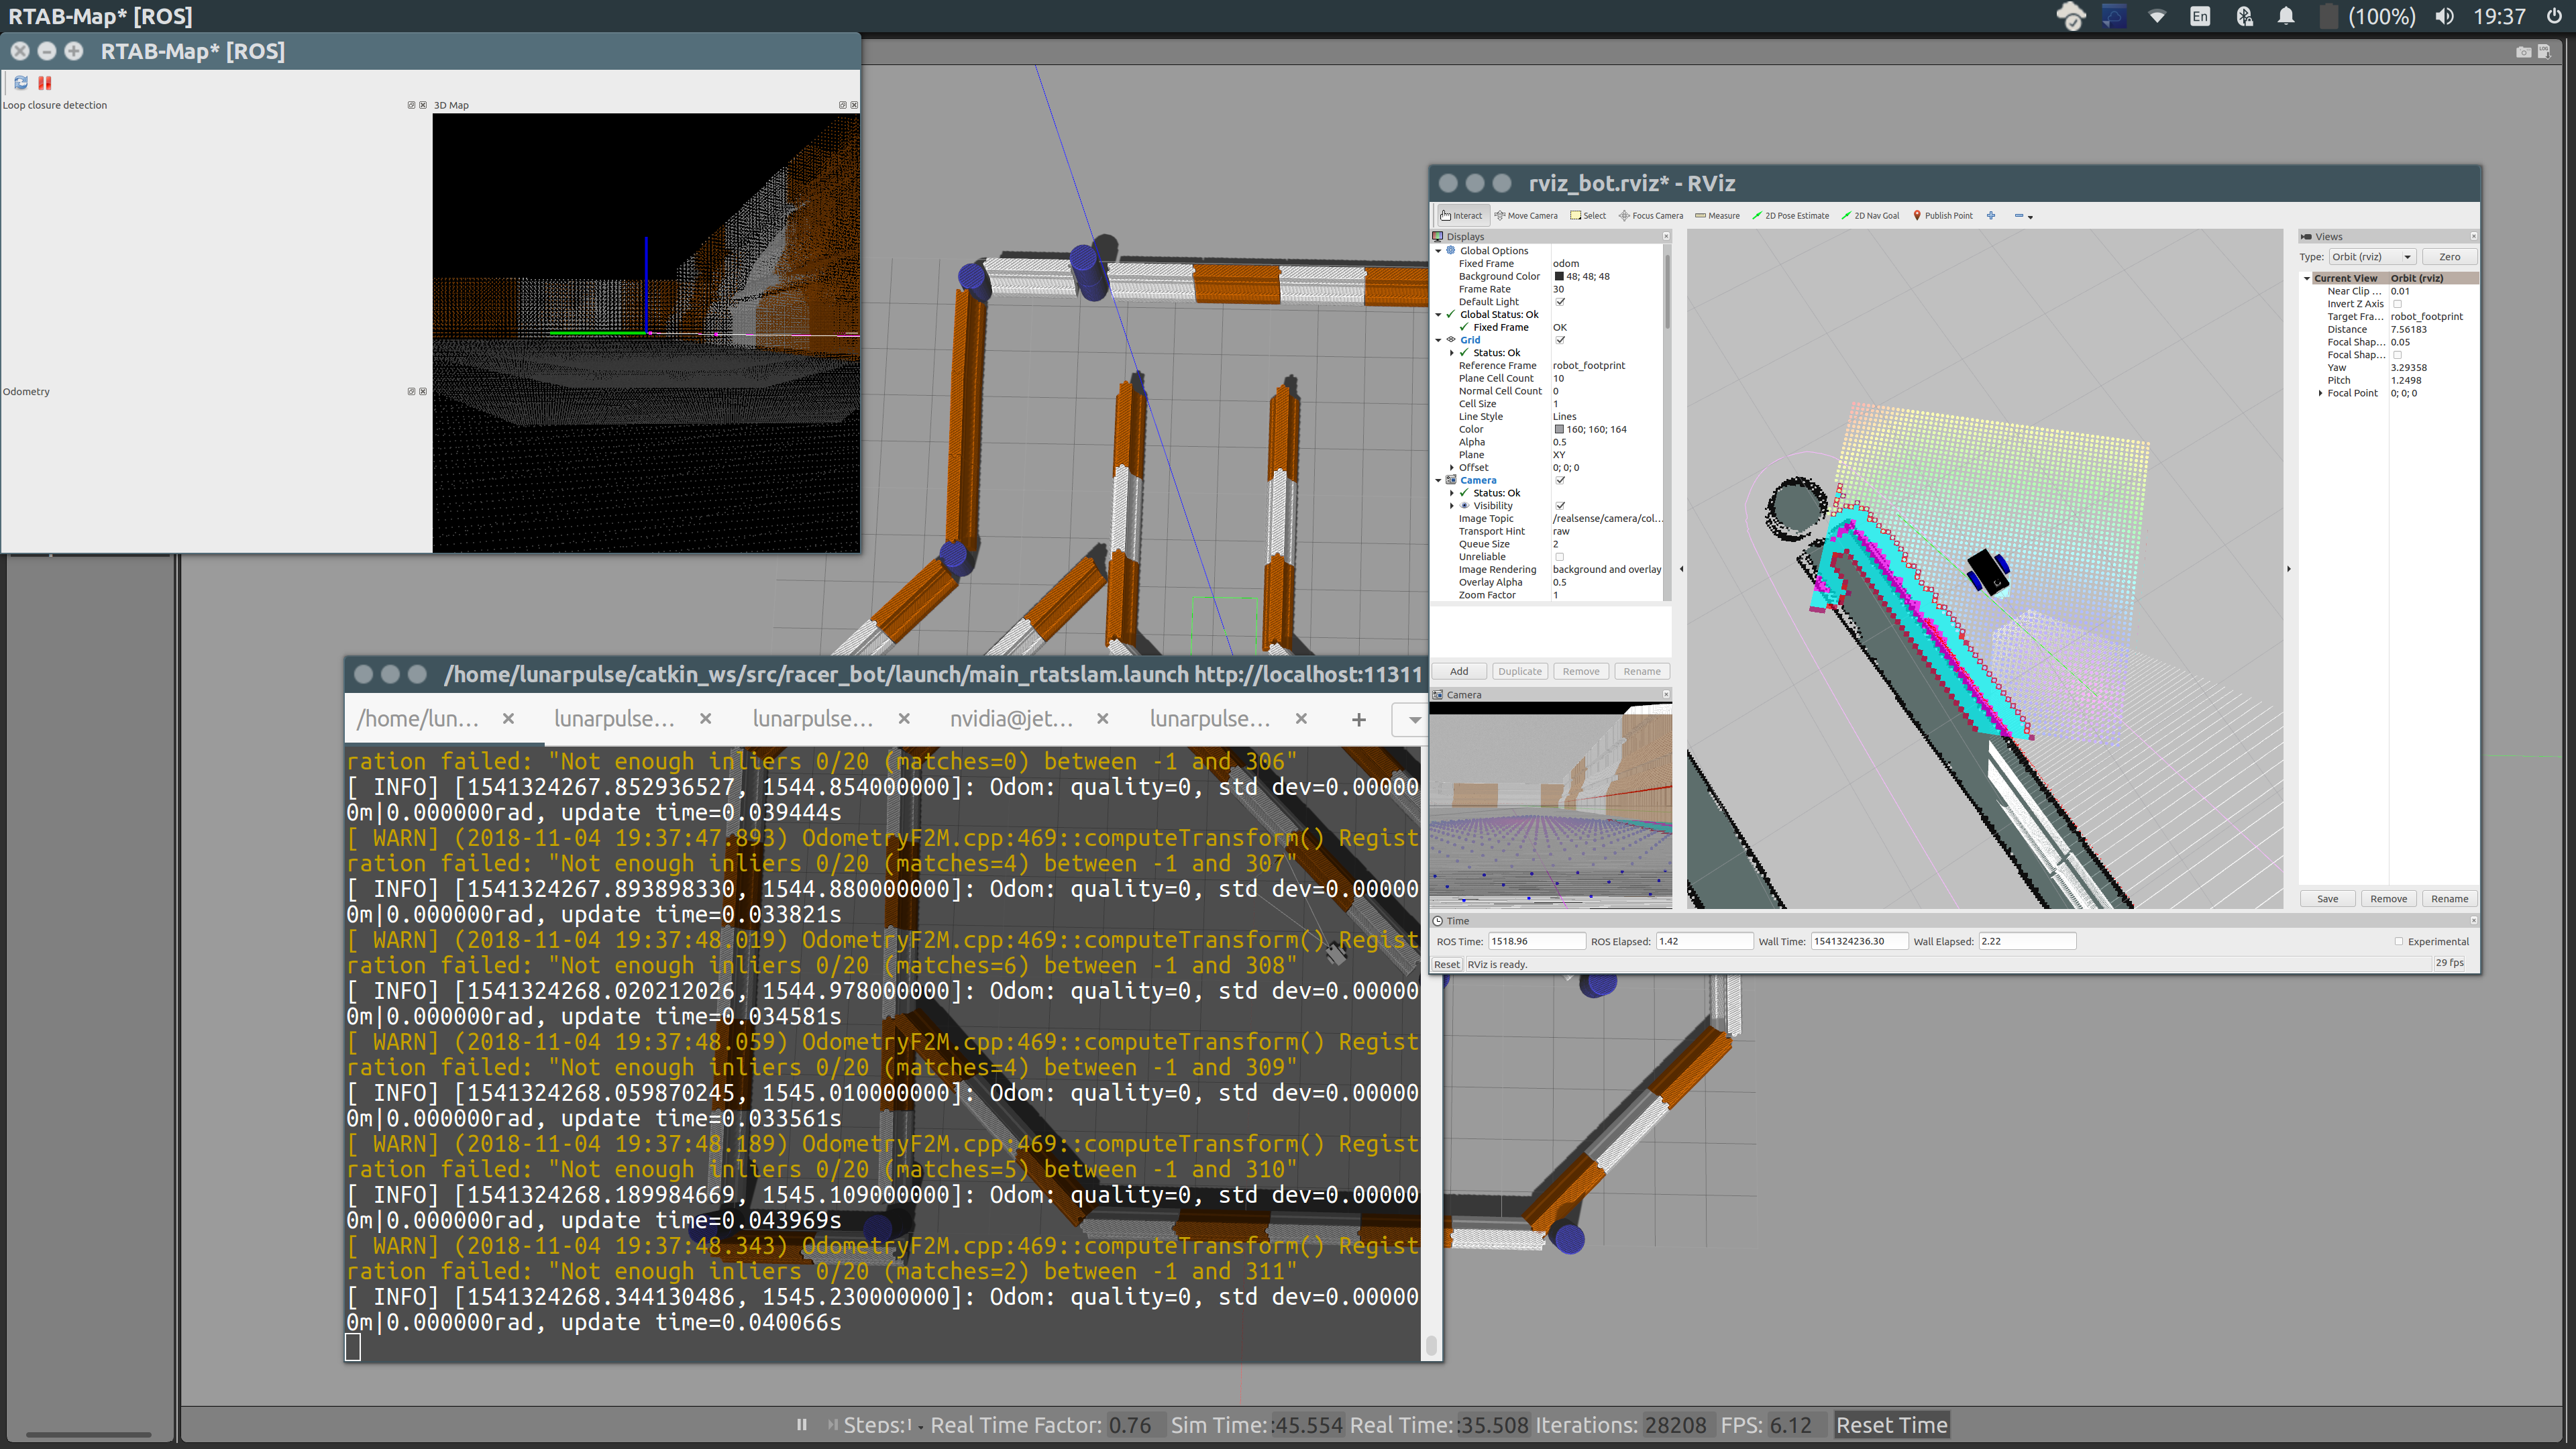
\includegraphics[width=\linewidth]{./img/rtabslam_racerbot.png}
      \caption{Screen shot with rtabslam}
      \label{fig:rtabslam_racerbot}
\end{figure}


\subsection{Technical Comparison} % only facts
Discuss the difference of the layout, parameters, performance etc. between the benchmark robot and your robot. It is acceptable for your custom robot to perform worse than the provided robot. The focus is on learning and understanding, not performance. 

\section{Discussion}

The localisation provided by the AMCL was intuitive and provided a successful localisation with small variance was achieved with the default values for its parameters. It is an easy use of the adaptive monte carlo localisation. The scattered arrows of estimated poses were gathered to the model of the robot in 5 seconds while navigating between the obstacles due to the observed obstacles in a continous manner, if it was in a place without any obstacles in a detectable range of the sensor, it takes a longer time to pin the pose of the robot. The cost cloud map also is related to the existance of local obstacles too.


\subsection{Questions}
\subsection{Which robot performed better?}
Which robot performed better? Same performance as the RTABSLAM map was not linked. Basically both use the static map from jakal. 
In addition, the code provided to test does not roam to make the global map first. It is possible to make a code let robot roaming in the environment without stuck, and then start the testing with the map created while wondering. However, this process is in SLAM part of the course, it was not sought after even though it is possible in theoretically.
\subsection{Why it performed better?}
In my opinion, the same physical shape and properties, inertia, there is no difference.
\subsection{How would you approach the 'Kidnapped Robot' problem?}
If global map is given, roaming purposely and infer the location using MCL is possible. If there is the array of distances to each landmark is given robot can localise itself with EKF or KF.I would go for simultaneous mapping and loclisation. The resason for my choice is that there is no way the robot would know where the robot is unless the global map is given at first. The robot should be able to make the map and navigate itself to the target position, if it can recognise target location in sight. 
\subsection{What types of scenario could localization be performed?}
Any type of scenario with unique obstacles or object in the scene. It was observed that robot tend to lose its confidence in no object area near the corners. Indeed, unique objects helps localisation so much as it is used as landmarks with high confidence.
\subsection{Where would you use MCL/AMCL in an industry domain?}
Definately, use in autonomos vehicles because these are the fields gains much focus thesedays. I am planning to use 3D MCL for my drones with custom sensors. The RGBD camera will serve as its smart eyes well.
However, this should be more than two dimension for flying robots and cars, including various service unmanned vehicles.


\section{Conclusion / Future work}

A variable processing mode for cluttered environment and non-obstacle mode can help this robot. In complicated and collision prone area or near the goal position, a processing with more accuracy can prevent the robot collision. However, a low accuracy mode can be the default processing mode and it can save resource and make the robot operating in a more robust manner.
The set of technology used in this project can apply to many fields operating on the ground with two wheels. Robot vaccum cleaners have the same sets of sensors and actuators except, the vaccum device and continers. This two wheeled mobile platform with accurate localisation can be used as the base vehicle or carrier for many different research too. The callenges in implementation of this platfrom from a simulation to the offline is to select actuators, and its control logic, to program the interface firmware to the control logic and to build and tune according to the hardware specification iteratively.

Porting the simulation to a real robot has challenges. The calculation of inertia of the real physical body of the robot, instead of assumming all axis of inertia is 0.1. This will influence the parameters of costmap as the acceleration and deceleration of the offline robot will be different from the simulation, not only the calculation of the inertia, the noise level from the sensor will vary depending on the operational condition, EKF needs to be taking it accounted.

Overall, processes of tuning consumed majority of time and the amount of effort to understand the dynamics among navigation, localisation, and physics of robot was considerable in developing this even tough refering to the guide. With growing popularity of machine learning, the reinforcement learning is considered to be the very topic which can substitute human tunner's effort with probablistic analysis of parameters and acheive higher performance in a short time. This was shown by alpha go zero, mastering condensed human knowledge of Go for 2000 years  practice in a week. With new or continously changing systems, assumming no prior knowledge or short time expiry knowledge, such model free reinforcement leanring should be more approperiate to apply than relying human effort, as human tends to make mistakes in those situation.


\subsection{Modifications for Improvement}
\begin{enumerate}
      \item completion of RTABMAP for localisation and navigation
      \item one rgbd camera without hokyuo LIDAR
      \item set it for higher speed movement
      \end{enumerate}
\subsection{Hardware Deployment}
\begin{enumerate}
\item Sparkfun chassis, encoders and more microcontrollers and its drivers
\item Rasberry pi if the nodelets are light otherwise Jetson Xavier mounting on it
\item Mounting Realsense D435 on it
\end{enumerate}

\bibliography{bib}
\bibliographystyle{ieeetr}

\end{document}
